%!TEX root = main.tex
To improve the reliability of the channel, Low Density Parity Check (LDPC) is implemented in this section. Its aim is to add redundancy to the information sent by the transmitter and use these additional bits to detect and correct errors. LDPC codes have the property that the generator and check matrices are sparse, which allows a lower complexity implementation.
\subsection{LDPC encoding and hard decoding}
Figure~\ref{fig:ldpcBER} illustrates the channel coding gain as a function of the number of iterations.
Hereafter, the information bits are coded using (256,128) LDPC.
\begin{figure}[htbp]
    \centering
    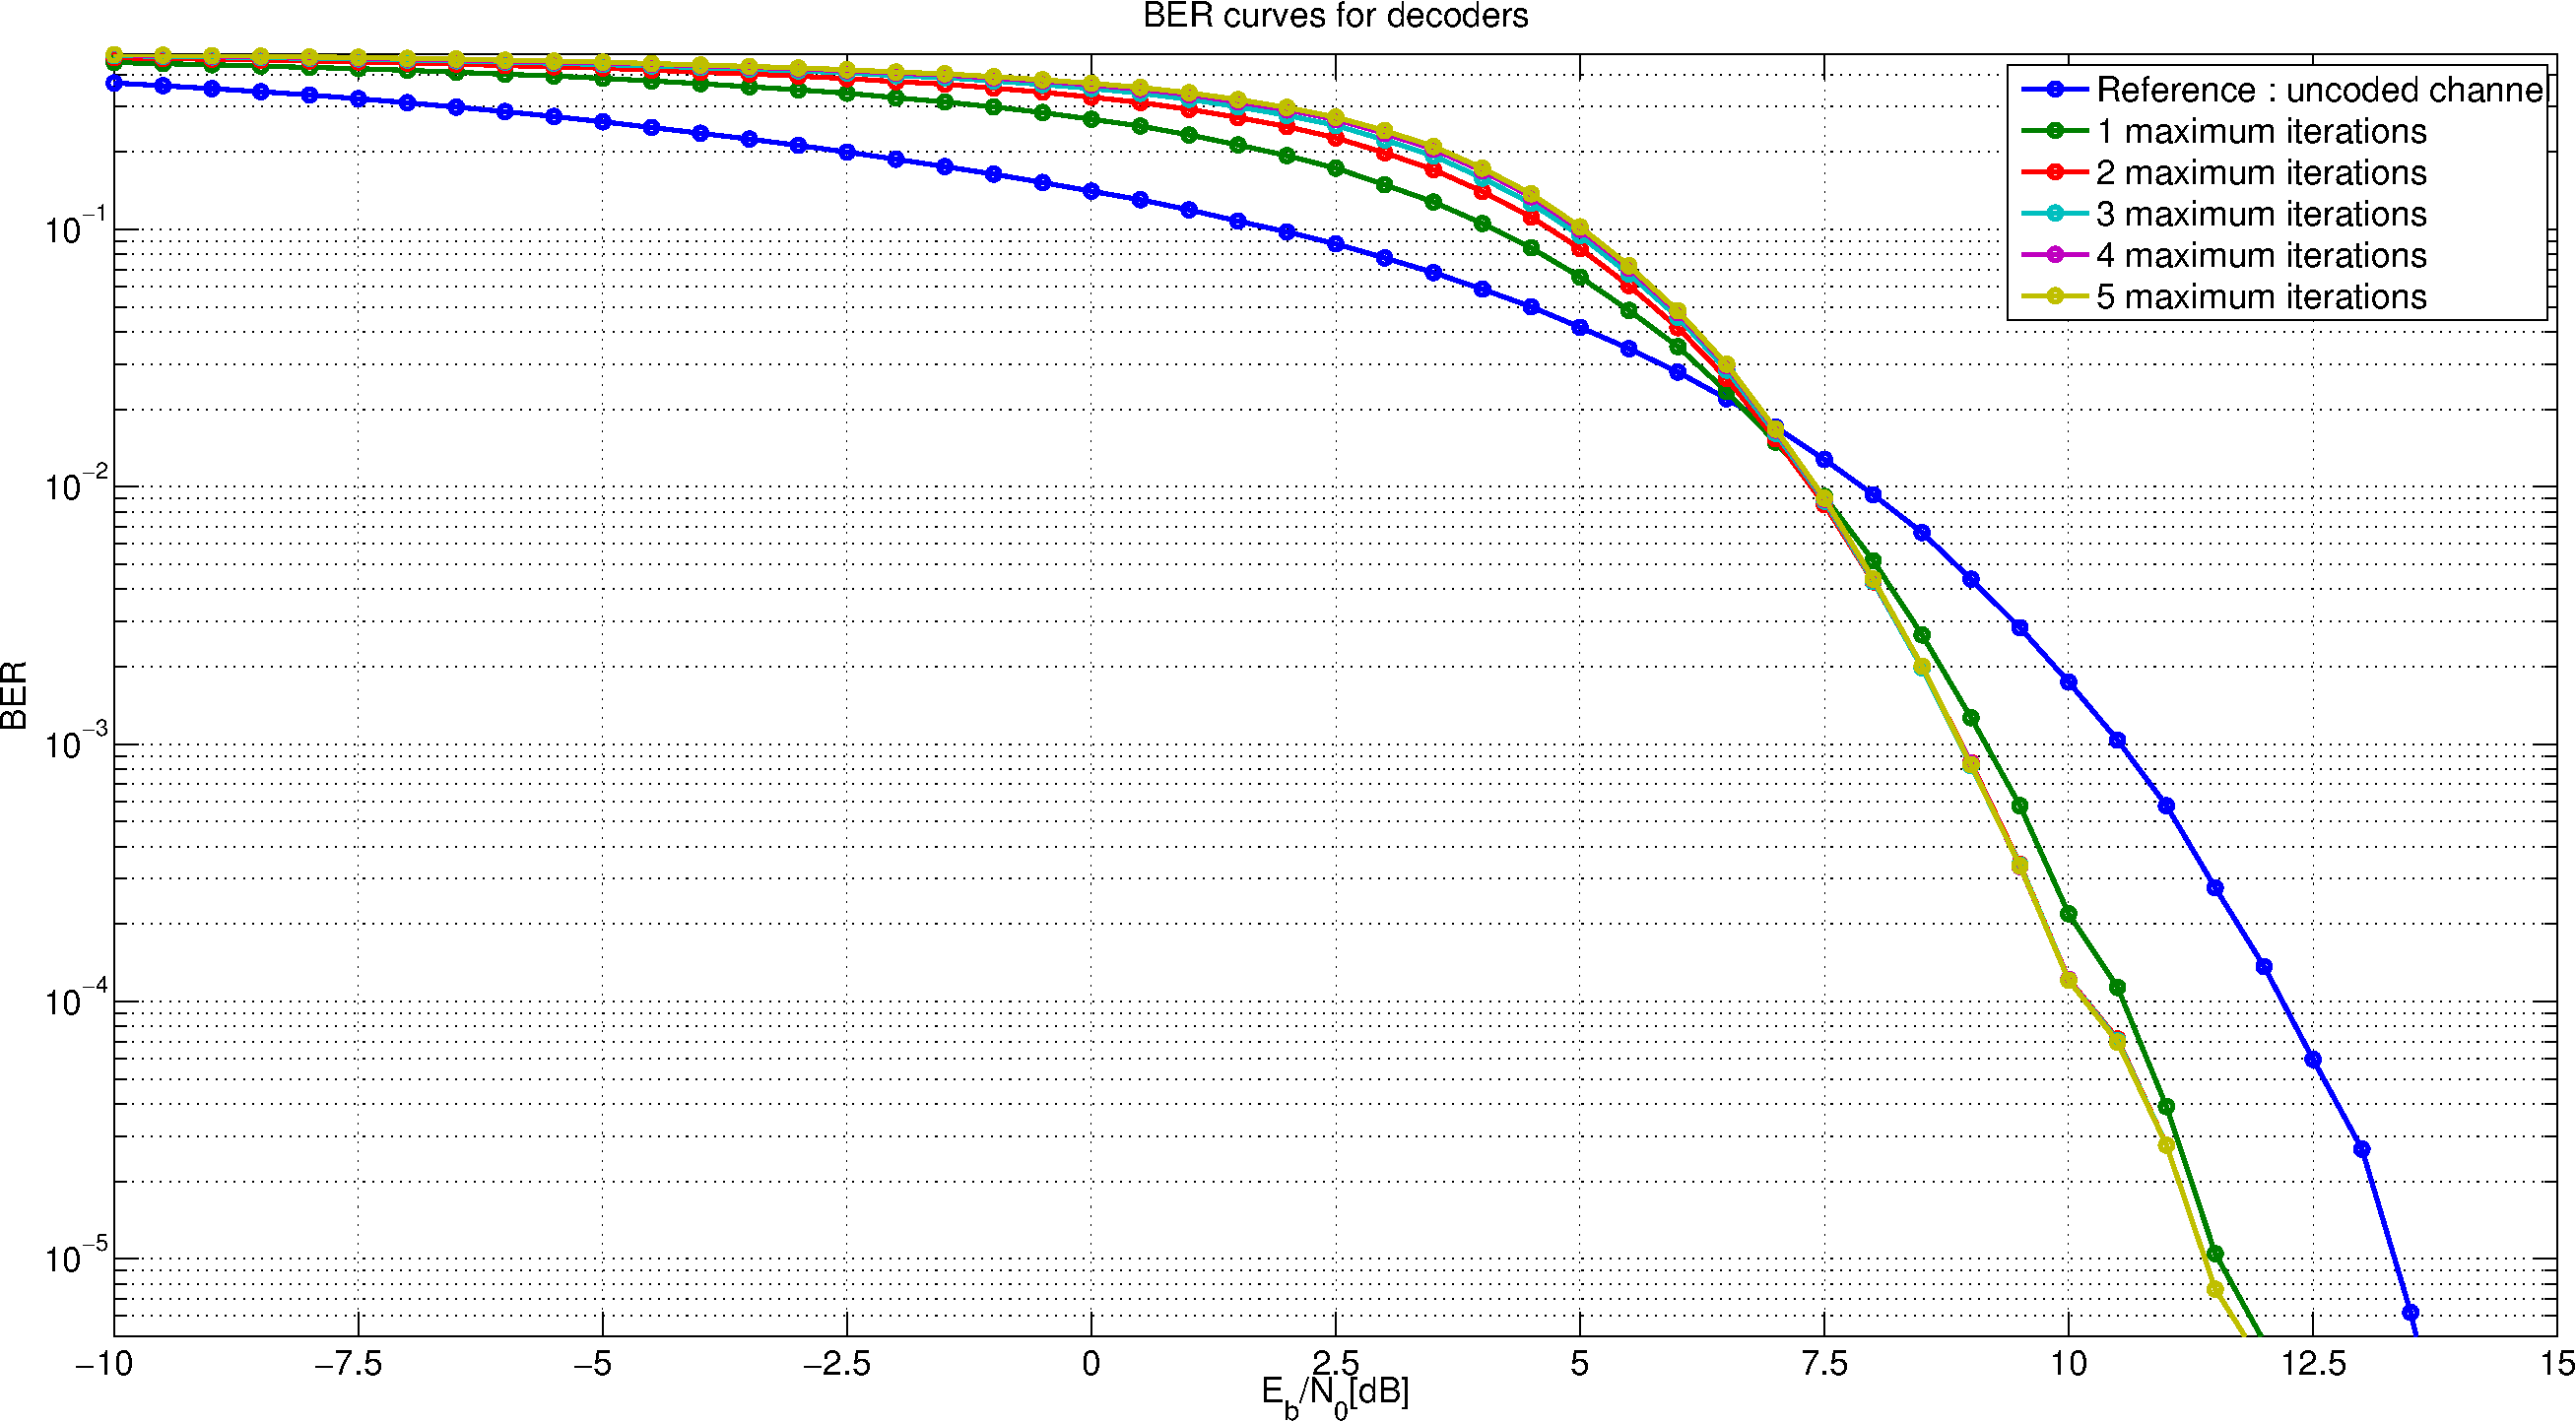
\includegraphics[width=\textwidth]{ldpcBER4.pdf}
    \caption{BER curves for different numbers of hard decoding iterations, compared with previous results.\label{fig:ldpcBER}}
\end{figure}

\subsection{Soft decoding}
Figure~\ref{fig:sldpcBER} compares the BER curves for the channel without coding, with coding and hard decoding and with different number of soft decoding iterations.
\begin{figure}[htbp]
    \centering
    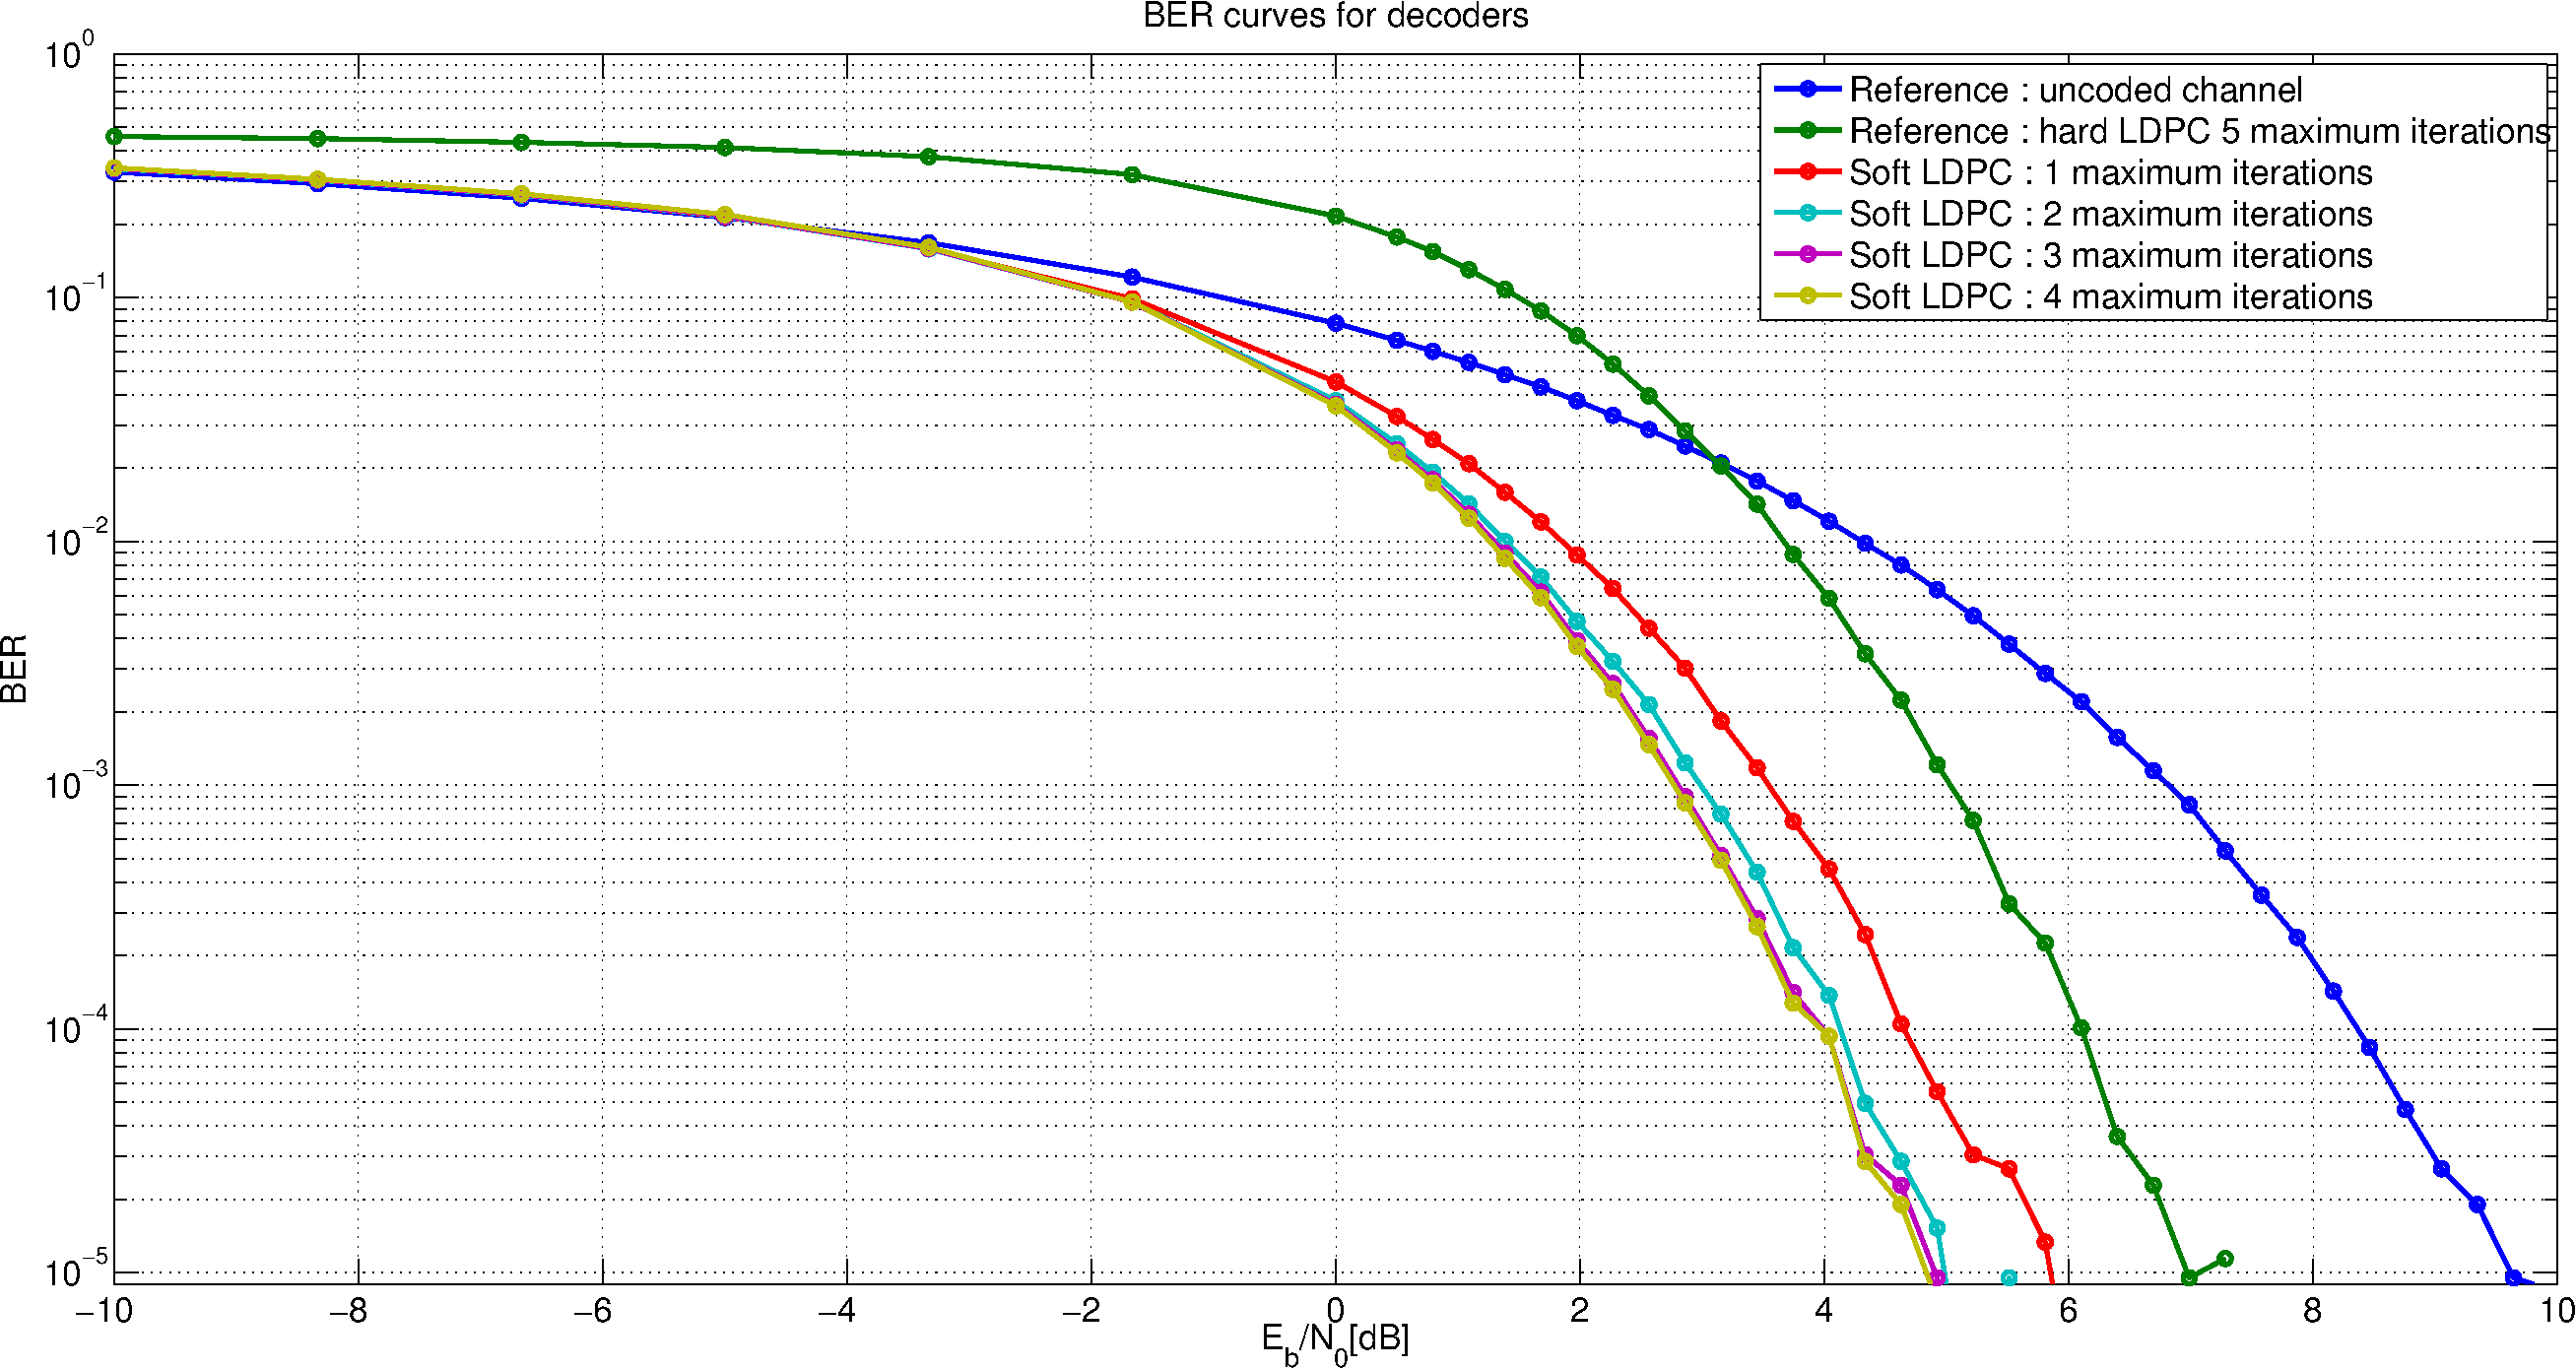
\includegraphics[width=\textwidth]{sldpcBER5.pdf}
    \caption{BER curves for different numbers of soft decoding iterations, compared with hard decoding and no coding.\label{fig:sldpcBER}}
\end{figure}
As will be explained in the next subsection, BPSK is used for this experiment.
We observe that, as expected, the soft decoder achieves better coding gain the the hard decoder. Moreover, it doesn't introduce additional errors at lower SNR. This is also due to how the decoder decides to stop iterating, since it stops iterating as soon as the number of detected errors increases.

\subsection{Questions}
\subsubsection{Simulation}
\paragraph{When building the new BER curves, do you consider the uncoded or coded bit energy on the x-axis?}
Here we consider the coded bit energy on the x-axis, but both options are interesting.
In a low-power application, the relevant metric is energy spent per sent bit of information in order to achieve a given error rate, which means the uncoded bit energy should be used on the x-axis.
If the emitter has constant power, the relevant metric is the coded bit energy which is defined as $\frac{P}{f_m \cdot \log_2(N_{sym})}$.

\paragraph{How do you limit the number of decoder iterations}
For hard decoding, the decoding stops as soon as one decoding iteration does not update the coded block, or when the maximum number of iterations is reached. This maximum number of iteration is set to 5. Figure~\ref{fig:ldpcBER} shows that very few additional errors are corrected past this value.
For soft decoding, the decoding stops as soon as there are no more detected errors, or when an iteration has actually introduced errors, or when the maximum number of iterations is reached.

\paragraph{Why is it much simpler to implement the soft decoder for BPSK or QPSK than for 16-QAM or 64-QAM?}
For BPSK and QPSK, there is no need to compare euclidean distances to the different points of the constellation. For BPSK, the probability that the received bit is a one or zero is simply given by the real part of the received symbol. For QPSK, the probability that the first bit is a one or zero is given by the real part of the received symbol, and the probability that the second bit is a one or a zero is given by its imaginary part.

\subsubsection{Communication system}
\paragraph{Demonstrate analytically that the parity check matrix is easily deduced from
the generator matrix when the code is systematic.}
A systematic code makes the information bits appear as is in the latter part of the coded block. Thus, the generator matrix can be written as $G = [P I]$. The parity check matrix is orthogonal to the generator matrix, so it must verify $G\cdot H^T = \overline{0}$. The solution to this identity is simply $H = [I P^T]$. Indeed:
\[
  [P I]\cdot[I P^T]^T = P \oplus P = \overline{0}
\]

\paragraph{Explain why we can apply linear combinations on the rows of the parity check matrix to
produce an equivalent systematic code.}
The important property of the parity check matrix is that it spans the vector subspace complementary to the codewords subspace spanned by the generator matrix. Linear combinations of the base vectors that form the columns of $H$ still span the same subspace, so it produces an equivalent code.

\paragraph{Why is it especially important to have a sparse parity check matrix (even more important
than having a sparse generator matrix)?}
Sparsity allows computational optimizations at various levels, but more specifically, it tremendously reduces the number of messages and responses between variable nodes and check nodes. This is because in the case of a sparse parity check matrix:
\begin{itemize}
  \item Each check node operates on a low number of variable nodes (few ones in every row).
  \item Each variable node intervenes in a low number of variable nodes (few ones in every column).
\end{itemize}

\paragraph{Explain why the check nodes only use the information received from the other variable
nodes when they reply to a variable node.}
In both hard- and soft-decoding, the messages exchanged between c-nodes and v-nodes must be stochastically independent. This means that when a node responds to another (regardless of the direction), it must only use extrinsic information, meaning that it shouldn't use the information from the node it is responding to.
